\documentclass[tikz,border=8pt]{standalone}
\usepackage{tikz}
\usetikzlibrary{positioning,calc,arrows.meta}
\usepackage{amsmath}
\usepackage{amssymb}

\definecolor{titledark}{RGB}{26,35,50}
\definecolor{lifeline}{RGB}{60,60,70}
\definecolor{honestgreen}{RGB}{27,94,32}
\definecolor{timeoutamber}{RGB}{230,126,20}
\definecolor{attackred}{RGB}{192,57,43}
\definecolor{bandgreen}{RGB}{223,237,222}
\definecolor{railgray}{RGB}{120,120,120}

\begin{document}
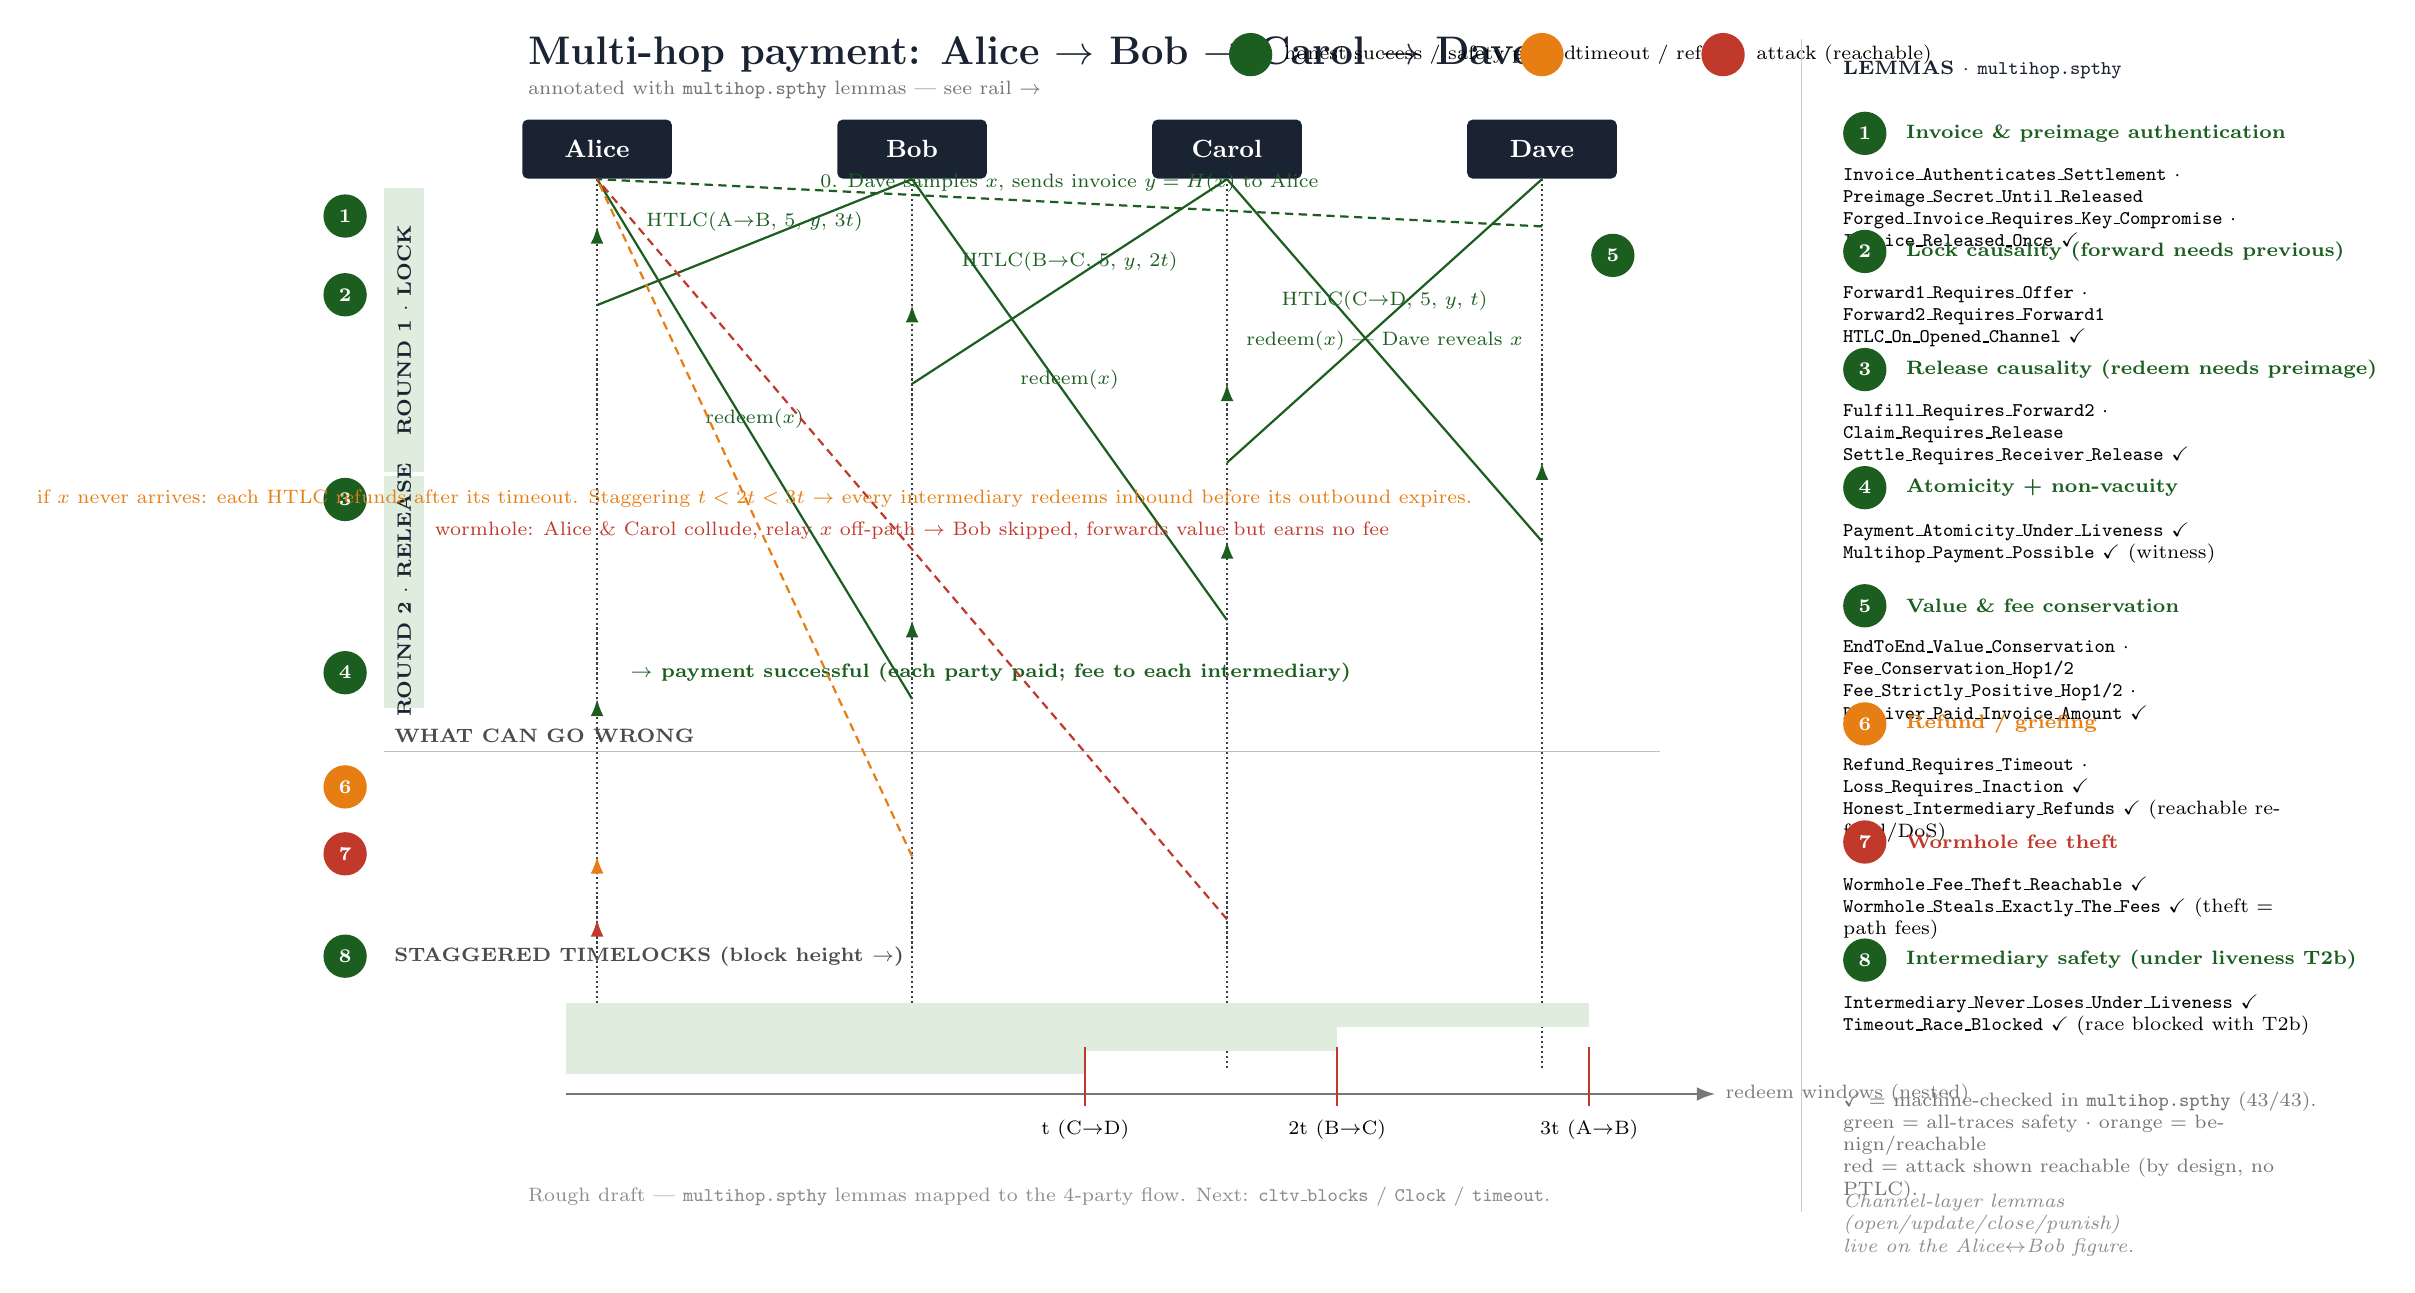
\begin{tikzpicture}[
  x=1cm, y=1cm,
  lifeline/.style={draw=lifeline, densely dotted, thick},
  headbox/.style={draw=none, fill=titledark, rounded corners=2pt,
                   minimum width=1.9cm, minimum height=0.75cm,
                   font=\bfseries\small, text=white},
  badge/.style={circle, draw=none, fill=#1, minimum size=0.55cm,
                font=\bfseries\scriptsize, text=white, inner sep=0pt},
  msg/.style={-{Latex[length=2.2mm]}, thick},
  msglab/.style={font=\scriptsize, align=center},
  legtitle/.style={font=\bfseries\scriptsize},
  legbody/.style={font=\scriptsize, align=left},
  roundband/.style={fill=bandgreen, draw=none}
]

% -------------------------------------------------------------------------
% Title + color key
% -------------------------------------------------------------------------
\node[anchor=west, font=\bfseries\Large, titledark] at (0,13.2)
  {Multi-hop payment: Alice $\to$ Bob $\to$ Carol $\to$ Dave};
\node[anchor=west, font=\scriptsize, black!55] at (0,12.75)
  {annotated with \texttt{multihop.spthy} lemmas --- see rail $\to$};

\node[badge=honestgreen] (keyg) at (9.3,13.2) {};
\node[anchor=west, font=\scriptsize] at (9.6,13.2) {honest success / safety proved};
\node[badge=timeoutamber] (keyo) at (13.0,13.2) {};
\node[anchor=west, font=\scriptsize] at (13.3,13.2) {timeout / refund};
\node[badge=attackred] (keyr) at (15.3,13.2) {};
\node[anchor=west, font=\scriptsize] at (15.6,13.2) {attack (reachable)};

% -------------------------------------------------------------------------
% Lifeline headers
% -------------------------------------------------------------------------
\node[headbox] (Alice) at (1.0,12.0) {Alice};
\node[headbox] (Bob)   at (5.0,12.0) {Bob};
\node[headbox] (Carol) at (9.0,12.0) {Carol};
\node[headbox] (Dave)  at (13.0,12.0) {Dave};

\draw[lifeline] (Alice.south) -- ++(0,-11.3);
\draw[lifeline] (Bob.south)   -- ++(0,-11.3);
\draw[lifeline] (Carol.south) -- ++(0,-11.3);
\draw[lifeline] (Dave.south)  -- ++(0,-11.3);

% -------------------------------------------------------------------------
% Round 1: LOCK  (y from 11.3 down to 8.3)
% -------------------------------------------------------------------------
\fill[roundband] (-1.7,7.9) rectangle (-1.2,11.5);
\node[rotate=90, font=\bfseries\scriptsize, titledark] at (-1.45,9.7) {ROUND 1 $\cdot$ LOCK};

\node[badge=honestgreen] (b1) at (-2.2,11.15) {1};
\draw[msg, honestgreen, densely dashed] (Dave.south -| Dave) ++(0,-0.6) --
  node[msglab, above, pos=0.5] {0. Dave samples $x$, sends invoice $y=H(x)$ to Alice}
  (Alice.south -| Alice) ++(0,-0.6);

\node[badge=honestgreen] (b2) at (-2.2,10.15) {2};
\draw[msg, honestgreen] (Alice.south -| Alice) ++(0,-1.6) --
  node[msglab, above, pos=0.5] {HTLC(A$\to$B, 5, $y$, 3$t$)}
  (Bob.south -| Bob) ++(0,-1.6);
\draw[msg, honestgreen] (Bob.south -| Bob) ++(0,-2.6) --
  node[msglab, above, pos=0.5] {HTLC(B$\to$C, 5, $y$, 2$t$)}
  (Carol.south -| Carol) ++(0,-2.6);
\draw[msg, honestgreen] (Carol.south -| Carol) ++(0,-3.6) --
  node[msglab, above, pos=0.5] {HTLC(C$\to$D, 5, $y$, $t$)}
  (Dave.south -| Dave) ++(0,-3.6);
\node[badge=honestgreen] (b5) at (13.9,10.65) {5};

% -------------------------------------------------------------------------
% Round 2: RELEASE  (y from 7.9 down to 5.2)
% -------------------------------------------------------------------------
\fill[roundband] (-1.7,4.9) rectangle (-1.2,7.85);
\node[rotate=90, font=\bfseries\scriptsize, titledark] at (-1.45,6.4) {ROUND 2 $\cdot$ RELEASE};

\node[badge=honestgreen] (b3) at (-2.2,7.55) {3};
\draw[msg, honestgreen] (Dave.south -| Dave) ++(0,-4.6) --
  node[msglab, above, pos=0.5] {redeem($x$) --- Dave reveals $x$}
  (Carol.south -| Carol) ++(0,-4.6);
\draw[msg, honestgreen] (Carol.south -| Carol) ++(0,-5.6) --
  node[msglab, above, pos=0.5] {redeem($x$)}
  (Bob.south -| Bob) ++(0,-5.6);
\draw[msg, honestgreen] (Bob.south -| Bob) ++(0,-6.6) --
  node[msglab, above, pos=0.5] {redeem($x$)}
  (Alice.south -| Alice) ++(0,-6.6);

\node[badge=honestgreen] (b4) at (-2.2,5.35) {4};
\node[font=\bfseries\scriptsize, honestgreen] at (6.0,5.35)
  {$\to$ payment successful (each party paid; fee to each intermediary)};

% -------------------------------------------------------------------------
% What can go wrong
% -------------------------------------------------------------------------
\node[anchor=west, font=\bfseries\scriptsize, black!70] at (-1.7,4.55) {WHAT CAN GO WRONG};
\draw[black!25] (-1.7,4.35) -- (14.5,4.35);

\node[badge=timeoutamber] (b6) at (-2.2,3.9) {6};
\draw[msg, timeoutamber, densely dashed] (Bob.south -| Bob) ++(0,-8.6) --
  node[msglab, above, pos=0.5, timeoutamber]
  {if $x$ never arrives: each HTLC refunds after its timeout. Staggering $t<2t<3t$ $\to$ every intermediary redeems inbound before its outbound expires.}
  (Alice.south -| Alice) ++(0,-8.6);

\node[badge=attackred] (b7) at (-2.2,3.05) {7};
\draw[msg, attackred, densely dashed] (Carol.south -| Carol) ++(0,-9.4) --
  node[msglab, above, pos=0.5, attackred]
  {wormhole: Alice \& Carol collude, relay $x$ off-path $\to$ Bob skipped, forwards value but earns no fee}
  (Alice.south -| Alice) ++(0,-9.4);

% -------------------------------------------------------------------------
% Staggered timelocks rail
% -------------------------------------------------------------------------
\node[badge=honestgreen] (b8) at (-2.2,1.75) {8};
\node[anchor=west, font=\bfseries\scriptsize, black!70] at (-1.7,1.75) {STAGGERED TIMELOCKS (block height $\to$)};

\fill[bandgreen] (0.6,0.85) rectangle (13.6,1.15);
\fill[bandgreen] (0.6,0.55) rectangle (10.4,0.85);
\fill[bandgreen] (0.6,0.25) rectangle (7.2,0.55);

\draw[railgray, thick, -{Latex}] (0.6,0.0) -- (15.2,0.0) node[right, font=\scriptsize] {redeem windows (nested)};
\foreach \x/\lab in {7.2/t (C$\to$D), 10.4/2t (B$\to$C), 13.6/3t (A$\to$B)} {
  \draw[attackred, thick] (\x,0.6) -- (\x,-0.15);
  \node[font=\scriptsize, below] at (\x,-0.2) {\lab};
}

\node[font=\scriptsize, black!55] at (7.2,-0.75) {};

% -------------------------------------------------------------------------
% Footer
% -------------------------------------------------------------------------
\node[anchor=west, font=\scriptsize, black!45] at (0,-1.3)
  {Rough draft --- \texttt{multihop.spthy} lemmas mapped to the 4-party flow. Next: \texttt{cltv\_blocks} / \texttt{Clock} / \texttt{timeout}.};

% ===========================================================================
% Legend panel (right side)
% ===========================================================================
\draw[black!20] (16.3,13.4) -- (16.3,-1.5);

\node[anchor=west, font=\bfseries\scriptsize, titledark] at (16.7,13.0)
  {LEMMAS $\cdot$ \texttt{multihop.spthy}};

\newcommand{\legitem}[5]{%
  % #1 = y-position (top), #2 = badge color, #3 = number, #4 = title, #5 = body
  \node[badge=#2] at (17.1,#1) {#3};
  \node[legtitle, anchor=west, text=#2] at (17.5,#1) {#4};
  \node[legbody, anchor=north west, text width=6.0cm] at (16.7,#1-0.32) {#5};
}

\legitem{12.2}{honestgreen}{1}{Invoice \& preimage authentication}
  {\texttt{Invoice\_Authenticates\_Settlement} $\cdot$ \texttt{Preimage\_Secret\_Until\_Released}\\
   \texttt{Forged\_Invoice\_Requires\_Key\_Compromise} $\cdot$ \texttt{Invoice\_Released\_Once} \checkmark}

\legitem{10.7}{honestgreen}{2}{Lock causality (forward needs previous)}
  {\texttt{Forward1\_Requires\_Offer} $\cdot$ \texttt{Forward2\_Requires\_Forward1}\\
   \texttt{HTLC\_On\_Opened\_Channel} \checkmark}

\legitem{9.2}{honestgreen}{3}{Release causality (redeem needs preimage)}
  {\texttt{Fulfill\_Requires\_Forward2} $\cdot$ \texttt{Claim\_Requires\_Release}\\
   \texttt{Settle\_Requires\_Receiver\_Release} \checkmark}

\legitem{7.7}{honestgreen}{4}{Atomicity + non-vacuity}
  {\texttt{Payment\_Atomicity\_Under\_Liveness} \checkmark\\
   \texttt{Multihop\_Payment\_Possible} \checkmark\ (witness)}

\legitem{6.2}{honestgreen}{5}{Value \& fee conservation}
  {\texttt{EndToEnd\_Value\_Conservation} $\cdot$ \texttt{Fee\_Conservation\_Hop1/2}\\
   \texttt{Fee\_Strictly\_Positive\_Hop1/2} $\cdot$ \texttt{Receiver\_Paid\_Invoice\_Amount} \checkmark}

\legitem{4.7}{timeoutamber}{6}{Refund / griefing}
  {\texttt{Refund\_Requires\_Timeout} $\cdot$ \texttt{Loss\_Requires\_Inaction} \checkmark\\
   \texttt{Honest\_Intermediary\_Refunds} \checkmark\ (reachable refund/DoS)}

\legitem{3.2}{attackred}{7}{Wormhole fee theft}
  {\texttt{Wormhole\_Fee\_Theft\_Reachable} \checkmark\\
   \texttt{Wormhole\_Steals\_Exactly\_The\_Fees} \checkmark\ (theft = path fees)}

\legitem{1.7}{honestgreen}{8}{Intermediary safety (under liveness T2b)}
  {\texttt{Intermediary\_Never\_Loses\_Under\_Liveness} \checkmark\\
   \texttt{Timeout\_Race\_Blocked} \checkmark\ (race blocked with T2b)}

\node[anchor=north west, font=\scriptsize, black!55, text width=6.3cm] at (16.7,0.15)
  {\checkmark\ = machine-checked in \texttt{multihop.spthy} (43/43).\\
   green = all-traces safety $\cdot$ orange = benign/reachable\\
   red = attack shown reachable (by design, no PTLC).};

\node[anchor=north west, font=\scriptsize\itshape, black!45, text width=6.3cm] at (16.7,-1.15)
  {Channel-layer lemmas (open/update/close/punish)\\
   live on the Alice$\leftrightarrow$Bob figure.};

\end{tikzpicture}
\end{document}
